\documentclass{beamer}
%pacchetti
\usepackage[T1]{fontenc}
\usepackage[utf8]{inputenc}
\usepackage{graphicx}
\usepackage[italian]{babel}
\usepackage{mathrsfs}
\usepackage{booktabs}
\usepackage{amsmath}
\usepackage{amsfonts}
\usepackage{amssymb}
\usepackage{amsbsy}
\usepackage{amsthm}
\usepackage{enumerate}
\usepackage{quoting}
\quotingsetup{font=small}
\usepackage{diagbox}
\usepackage{graphicx}
\usepackage{setspace}
\usepackage{float}
\usepackage{version}
\usepackage{multicol}
\usepackage{beamerfoils}

\usepackage{tikz}
\usepackage{lmodern}
\usepackage[absolute,overlay]{textpos}
\setbeamercolor{block body example}{fg=black,bg=blue} 
\setbeamercolor{block title example}{bg=black}

\usepackage[none]{hyphenat} %avoid hyphenation
\usepackage{xcolor} %to uset \textcolor
\usepackage{bbm} %funzione indicatrice
% end pacchetti

\usetheme[bgphoto]{polimi}

% Full instructions available at:
% https://github.com/elauksap/beamerthemepolimi

% Set custom font (requires to compile with XeLaTeX).
\usepackage{ifxetex}
\ifxetex
\usepackage{fontspec}
\setsansfont[Scale=0.9]{Arial}
\fi

\usepackage{lipsum}


\newcommand\mynum[1]{%
	\usebeamercolor{enumerate item}%
	\tikzset{beameritem/.style={circle,inner sep=0,minimum size=2ex,text=enumerate item.bg,fill=enumerate item.fg,font=\footnotesize}}%
	\tikz[baseline=(n.base)]\node(n)[beameritem]{#1};%
}


\title{Coupled Markov chains with applications to Approximate Bayesian Computation for model based clustering}
%\subtitle{Subtitle}
\author{E. Bertoni, M. Caldarini, F. Di Filippo, G. Gabrielli, E. Musiari}
\date{15 February 2022}


%Cose da fare

% Mettere biografia
% Mettere \pause e colori
% Sistemare il titolo e layout

\begin{document}
	
	\begin{frame}
		\maketitle
	\end{frame}
	
	\section{Introduction}
		
		\begin{frame}
			\frametitle{A complex problem}
			
			\begin{minipage}{0.45\textwidth}
				\begin{center}
					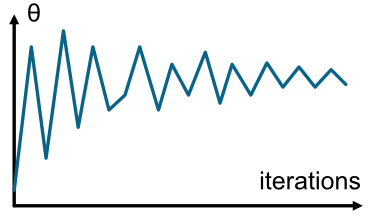
\includegraphics{img/markov_singola}
				\end{center}
			\end{minipage}
			\hfill
			\begin{minipage}{0.45\textwidth}
				\begin{center}
					
\includegraphics{img/likelihood_na}
				\end{center}
			\end{minipage}
			
			\vspace{0.5cm}
			
			\begin{minipage}{0.45\textwidth}
				\begin{center}
					$\Downarrow$
					
					\textbf{Unbiased Markov chain Monte Carlo methods with couplings}
				\end{center}
			\end{minipage} %}
			\hfill
			\begin{minipage}{0.45\textwidth}
				\begin{center}
					$\Downarrow$
					
					\textbf{Approximate Bayesian Computation}
				\end{center}
			\end{minipage} %}
			
			\vspace{0.2cm}
			
			\begin{minipage}{0.45\textwidth}
				\begin{center}
					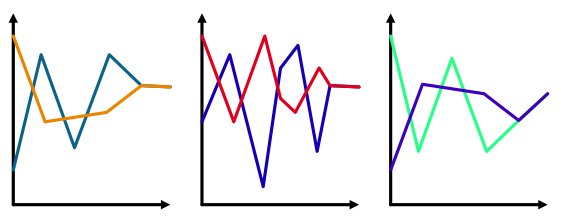
\includegraphics{img/markov_coupled_parallel}
				\end{center}
			\end{minipage}%}
			\hfill
			\begin{minipage}{0.45\textwidth}
				
			\end{minipage}
			
			
			
		\end{frame}
		
	
	


\section{The complete method: MCMC + Couplings + ABC}
	
	\begin{frame}[plain]{}
		\sectionpage
	\end{frame}
	
	\begin{frame}
		\frametitle{Implementation}
		\begin{center}
			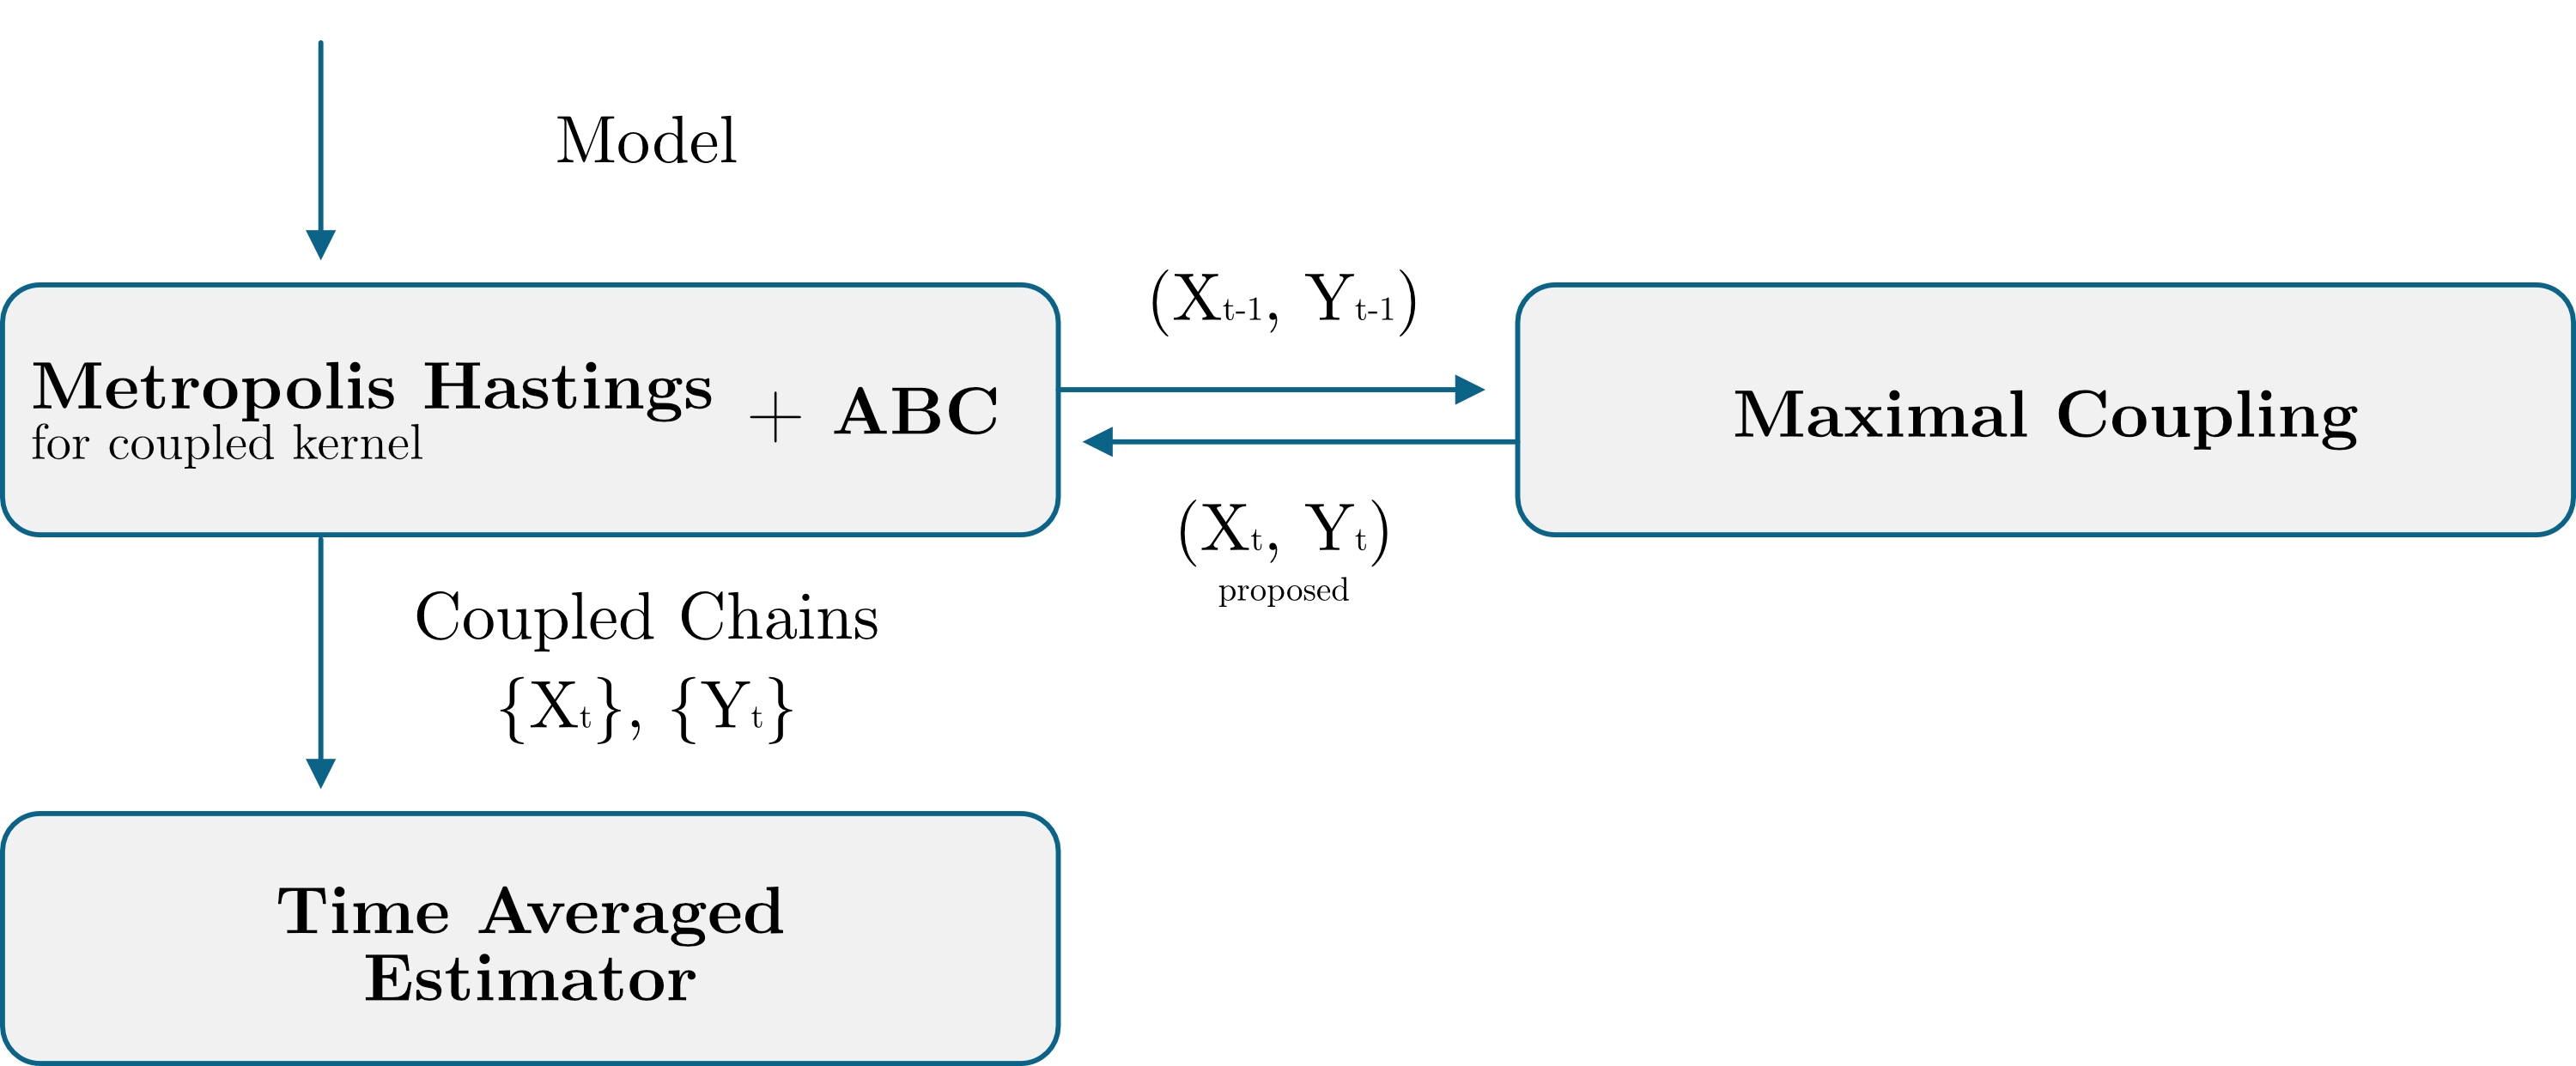
\includegraphics[width=\textwidth]{img/Bayes3}
		\end{center}
	\end{frame}
%------------------------------------------------
	\begin{frame}
	\frametitle{Maximal coupling}
	Maximal coupling between two distributions p and q 
%	Set $p = \mathcal{N}(X_{t-1},0.1^2)$ and $q = \mathcal{N}(Y_{t-1},0.1^2)$, then:
	\begin{itemize}
		\item sample $X \sim p$;
		\item sample $W|X \sim \mathcal{U}\{[0,p(X)]\}$;
		\item if $W\leq q(X)$ then output $(X,X)$, otherwise:
		\begin{enumerate}
			\item sample $Y \sim q$;
			\item sample $W^\star | Y \sim \mathcal{U}\{[0, q(Y)]\}$ 
			until $W^\star > p(Y)$ 
			\item output $(X,Y)$.
		\end{enumerate}
	\end{itemize}
\begin{block}{Output}
		 Distribution of a pair of random variables X, Y that maximizes $\mathbb{P}(X=Y)$
		 subject to the marginal constraints $X \sim p$ and $Y \sim q$
	
\end{block}
\end{frame}
%------------------------------------------------------------------------------------
	\begin{frame}
		\frametitle{Metropolis Hastings with couplings and ABC}
		\begin{block}{Model}
				
				$$ Y_i | \mu, \sigma^2 \overset{iid}{\sim} \mathcal{N}(\mu, \sigma^2) $$
				$$ \mu  \sim \mathcal{N}(\mu_0, \sigma_0^2)  $$
				$$ \sigma^2  \sim InvGa(a,b) $$
				
			
		\end{block}
	%	$$ \pi( \boldsymbol{\theta}) =\pi(\mu)*\pi(\sigma) $$
		$$ \mu_0 = 8, \quad \sigma^2_0 = 4$$
		$$ a=b=1 $$
		
	\end{frame}
%------------------------------------
\begin{frame}
	\frametitle{Metropolis Hastings with couplings and ABC}
	\only<1>{
		\begin{block}{}
			\begin{center}
			\textbf{Initilization} 
			\end{center}
		\end{block}	
	set $\boldsymbol{\theta}=(\mu,\sigma^2)$\\
	
			for k=1,2:
			
			until $K_h(||s_{k}^{(0)}-s_{obs}||)>0$:
	\begin{itemize}
				
		\item sample $\boldsymbol{\theta}_{k}^{(0)} \sim  \pi(\boldsymbol{\theta})$  
		\item simulate $n_{obs}$ observations $y_{ki} \sim \mathcal{N}(\mu^{(0)},\sigma^{2(0)})$ from  maximal coupling 
		\item compute $s_{k}^{(0)}=S(y_{k})$ ;
	\end{itemize}
		
			
	
	}
	\only<2>{
		\begin{block}{}
			\begin{center}
				\textbf{Iterations} 
			\end{center}
	\end{block}	
			 for i = 1,...,M:
			
			given $\boldsymbol{\theta}^{(i-1)}=(\mu^{(i-1)},\sigma^{2(i-1)})$
			\begin{itemize}
				
				\item generate [$\boldsymbol{\theta}_{1}^{(i)},\boldsymbol{\theta}_{2}^{(i)}$] from a maximalcoupling given [$\boldsymbol{\theta}_{1}^{(i-1)},\boldsymbol{\theta}_{2}^{(i-1)}$];
				
				\item for k=1,2:
				\begin{enumerate}
				\item simulate $n_{obs}$ observations $y_{k}^{(i)} \sim \mathcal{N}(\mu^{(i)},\sigma^{2(i)})$ from  maximal coupling;
				\item compute $s_{k}^{(i)}=S(y_{k})$;
				\item accept $\boldsymbol{\theta}_{k}^{(i)}$ with probability 
				$$
				\frac{
					K_h(||s_{k}^{(i)}-s_{obs}||)\pi(\boldsymbol{\theta}_{k}^{(i)})
				}{
					K_h(||s_{k}^{(i-1)}-s_{obs}||)\pi(\boldsymbol{\theta}_{k}^{(i-1)})
				}
				$$
				\end{enumerate}
				
			\end{itemize}
			
		

	}
	\only<3>{
		\begin{block}{}
			\begin{center}
			\textbf{Output}
			\end{center}
		\end{block}
			for k= 1,2
		$$\mu_{k}^{(1)},...,\mu_{k}^{(M)}\sim \pi_{ABC} (\mu|y_{obs});$$
		$$\sigma_{k}^{2(1)},...,\sigma_{k}^{2(M)} \sim \pi_{ABC} (\sigma|y_{obs}).$$
	}

\end{frame}
%-----------------------------------

	
\begin{frame}
	\frametitle{Study case}
	
	\textbf{Summary statistics}: Sample mean, Sample Variance \\


	\textbf{Distance}: $L^2-norm$
	%malanobis nel multivariato
	
	\textbf{Kernel}: $
	K(u) = 
	\frac{1}{\sqrt{2\pi}} e^{-\frac{1}{2} u^2}, 
	\quad K_h(u) 
	= \frac{K(\frac{u}{h})}{h}
	$
	%1/(np.sqrt(2*math.pi))np.exp(-1/2*u*2)		

	\textbf{Proposal distribution}:	$	% \begin{bmatrix}    % non so perchè non vada
%	\mu' \\ log(\sigma^2 ')	\end{bmatrix} 
	\sim \mathcal{N}\left( \begin{bmatrix}    % non so perchè non vada
	\mu^{(i)} \\ log(\sigma^{2(i)})
	\end{bmatrix}, 0.1^2 \cdot\mathcal{I}\right)$
	%	\hspace*{4cm}	$  y' \sim \mathcal{N}(\mu^{(i)} , \sigma^{2(i)})$

\pause

	
	\begin{block}{Dataset}
	
	100 samples generated from a Gaussian distribution:
		
		$$ Y_{obs} \sim \mathcal{N}(\mu_{obs}, \sigma_{obs}^{2}) $$
		$$	\mu_{obs} = 10,	\sigma_{obs}^{2} = 3	$$
	
	\end{block}
\end{frame}
	
%-------------------------------------------------------------------
\begin{frame}
	\frametitle{Results for parameter $\mu$}
	\begin{columns}
		\begin{column}{0.4\textwidth}
		{\scriptsize \textbf{Coupled chains from one processor}}\\
		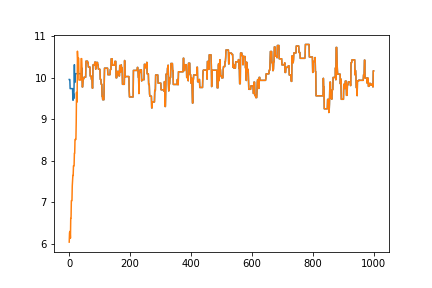
\includegraphics[width=6cm,height=2.3cm]{doublecoupling_chainmeeting/doublecoupling_mu_chain_meeting}
		\vspace{0.2cm}
	{	\scriptsize \textbf{Samplings from all accepted chains }}\\
	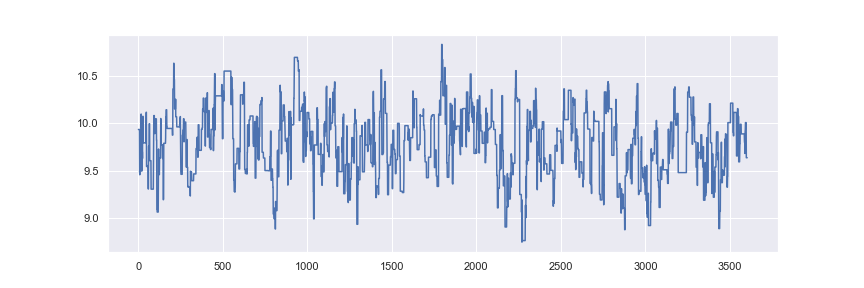
\includegraphics[width=6cm,height=2.3cm]{doublecoupling_pack/doublecoupling_sampling_mu}
		%						%	
		\end{column}
	\begin{column}{0.4\textwidth}
		{\scriptsize \textbf{Sampling histogram with estimated distribution}}\\
		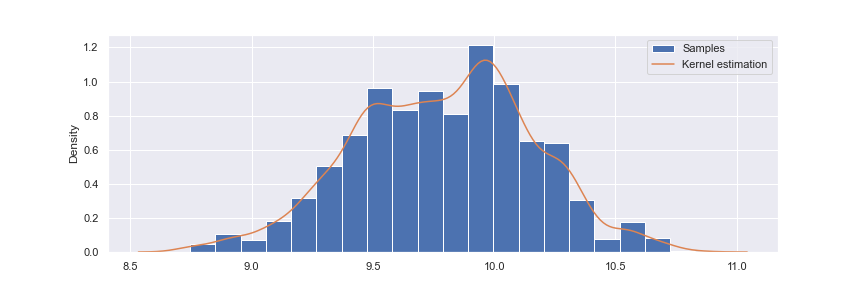
\includegraphics[width=6cm,height=5cm]{doublecoupling_pack/doublecoupling_mu_histogram_kernel}
	\end{column}
	\end{columns}

	\small
	Time Averaged Estimators mean obtained:	$ \mathbb{E}[H_{k:m}(X_{\mu}, Y_{\mu})] \simeq 9.8   % non so perchè non vada
	$
	
	
	
\end{frame}
\begin{frame}
	\frametitle{Results for parameter $\sigma^2$}
	\begin{columns}
		\begin{column}{0.4\textwidth}
			{\scriptsize \textbf{Coupled chains from one processor}}\\
			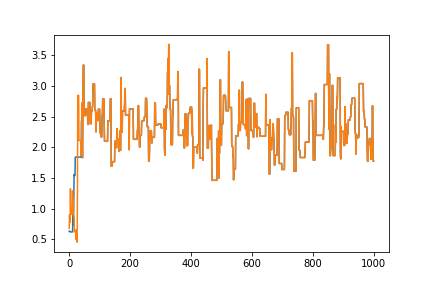
\includegraphics[width=6cm,height=2.3cm]{doublecoupling_chainmeeting/doublecoupling_sigma_chain_meeting}
			\vspace{0.2cm}
			{	\scriptsize \textbf{Samplings from all accepted chains }}\\
			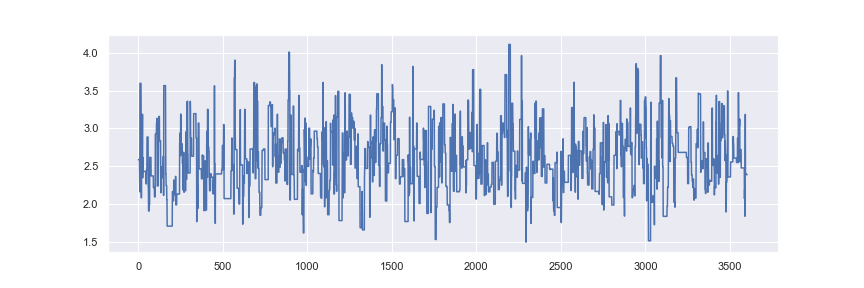
\includegraphics[width=6cm,height=2.3cm]{doublecoupling_pack/doublecoupling_sampling_sigma}
			%						%	
		\end{column}
		\begin{column}{0.4\textwidth}
			{\scriptsize \textbf{Sampling histogram with estimated distribution}}\\
			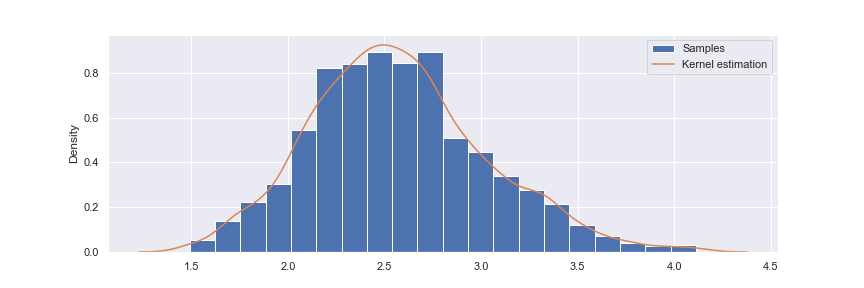
\includegraphics[width=6cm,height=5cm]{doublecoupling_pack/doublecoupling_sigma_histogram_kernel}
		\end{column}
	\end{columns}
	
	\small
	Time Averaged Estimators mean obtained:$\mathbb{E}[H_{k:m}(X_{\sigma^2}, Y_{\sigma^2})] \simeq 2.56   % non so perchè non vada
	$
	
\end{frame}

%---------------------------------------------------------------------------------
	
\section{Numerical experiment: g-and-k distribution}

\begin{frame}[plain]{}
	\sectionpage
\end{frame}
	\begin{frame}
		\frametitle{Model}
		\begin{block}{Quantile function}
			
			$$ r \in (0,1) \longmapsto   a + b (1+0.8\left(\frac{1-exp(-g \cdot z(r))}{1+exp(-g\cdot z(r))}\right)(1+ z(r)^{2})^k\cdot z(r)  $$
		\end{block}	
		where $ z(r)$ is the r-th quantile of the standard Normal distribution. 
		\begin{block}{Prior distributions}
			$$ a \sim \mathcal{U}([0,10])	$$
			$$ b \sim \mathcal{U}([0,10])	$$
			$$ g \sim \mathcal{U}([0,10])	$$
			$$k \sim \mathcal{U}([0,10])    $$
		\end{block}
	\end{frame}
	
	
	
	\begin{frame}
		\frametitle{Study case}
		
		\textbf{Summary statistics}: 10 quantiles
			
		\textbf{Distance}: $ L^2-norm $
			
		\textbf{Kernel}: 
		$$
		K(u) = 
		\frac{1}{\sqrt{2\pi}} e^{-\frac{1}{2}u^2}, 
		\quad K_h(u) 
		= \frac{K(\frac u h)}{h}
		$$
		%1/(np.sqrt(2*math.pi))np.exp(-1/2*u*2)
		
	\begin{columns}
		\begin{column}{0.6\textwidth}
		\begin{block}{Dataset}
			100 samples generated as follows:
			$$a_{obs}= 3 ,
			 b_{obs}= 1 ,
			 g_{obs}=2 ,
			 k_{obs}=0.5 $$
			$$ y_{obs} \sim quantilefunction(z(r), \theta_{obs})$$
			$$ z(r) \sim \mathcal{N}(0,1)$$
%			$$	y_{obs} =a_{obs} + b_{obs} (1+0.8\left(\frac{1-exp(-g_{obs}\cdot z(r))}{1+exp(-g_{obs}\cdot z(r))}\right)(1+z(r)^{2})^k\cdot z(r)	$$
%			and $$ z(r) \overset{iid}{\sim} \mathcal{N}(0,1) $$
			
		\end{block}
		\end{column}
	\begin{column}{0.3\textwidth}
		%\begin{minipage}{0.\textwidth}
			
			\begin{center}
				{\scriptsize \textbf{Quantile distribution: $y_{obs}$}}
				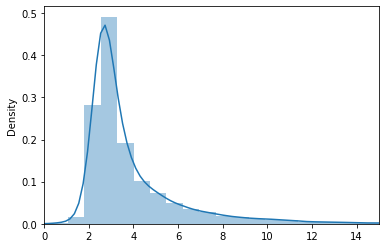
\includegraphics[width=4cm,height=3cm]{immagini_mario/density_quantile}
			\end{center}
	%	\end{minipage}
		\end{column}
	
	\end{columns}
		
	\end{frame}
%---------------------------------------------------------------
\begin{frame}{Metropolis Hastings with couplings and ABC}


	\begin{block}{}
		\begin{center}
			\textbf{Initialization} 
		\end{center}
	\end{block}	
	given $\theta =( a,b,g,k )$
	
	for k=1,2:
	
	 Untill $K_h(\|s_{k}^{(0)} - s_{obs}\|)>0$:
		\begin{itemize}
			\item Generate $\theta_{k}^{(0)} \sim \mathcal{U}([0,10]^4)$ from prior density.
			\item Generate $z(r) \sim \mathcal{N}(0,1)$
			\item Generate a sample of $n_{obs}$ observations such that $y_{k} \sim quantile function(z(r),\theta_{k}^{0})$
			\item Compute $s_{k}^{(0)}=S(y_{k})$
			
		\end{itemize}

	

		
		\end{frame}
	\begin{frame}{Metropolis Hastings with couplings and ABC}
	
		\begin{block}{}
			\begin{center}
				\textbf{Iterations} 
			\end{center}
		\end{block}	
		
		for i in (1,...,M):
		\begin{itemize}
			\item generate $\theta_{1}^{(i)},\theta_{2}^{(i)}$  from maximalcoupling$(\theta_{1}^{(i-1)},\theta_{2}^{(i-1)})$
			
			\item \textcolor{red}{simulate $n_{obs}$ observations $ y_{1}^{(i)}$,$ y_{2}^{(i)}$ from maximal coupling}
				
				
		
			\item Compute the summaries  $ s_{k}^{(i)} =S(y_{k}^{(i)})$ 
			
			
			\item Accept $\theta_{k}^{(i)}$ with probability $$\frac{Kh(\|s_{k}^{(i)}-s_{obs}\|)\pi(\theta_{k}^{(i)})}{Kh(\|s_{k}^{(i-1)}- s_{obs}\|)\pi(\theta_{k}^{(i-1)})} $$   otherwise $\theta_{k}^{(i)}=\theta_{k}^{(i-1)}$;
			
			
		\end{itemize}
%		\only<2>{
%		\begin{textblock*}{\textwidth}
%			\begin{beamercolorbox}[wd=.5\textwidth,center,sep=0.3cm]{block body example}
%				
%				for j in (1,...,$n_{obs}$):
%				
%				
%			\end{beamercolorbox}
%		\end{textblock*}
%	}
	\only<2>{
		\begin{textblock*}{300pt}(30pt,80pt)%{\textwidth}(0.1\textwidth,0.1\textheight)
			\begin{block}{Couplings}
					 for j in (1,...,$n_{obs}$):
					\begin{enumerate}
						\item $z^{(i,j)}(r) \sim \mathcal{N}(0,1)$
						\item generate:
						$$ y_{1}^{(ij)} \sim quantile function(z^{(i,j)}(r), \theta_{1}^{(i-1)})$$
						$$ y_{2}^{(ij)} \sim quantile function(z^{(i,j)}(r), \theta_{2}^{(i-1)})$$
						
					\end{enumerate}
			\end{block}
		\end{textblock*}
	}
	\end{frame}

%------------------------------------------------------------------
\begin{frame}
	\frametitle{Results for parameter a}
	\begin{columns}
		\begin{column}{0.4\textwidth}
			{\scriptsize \textbf{Coupled chains from one core}}\\
			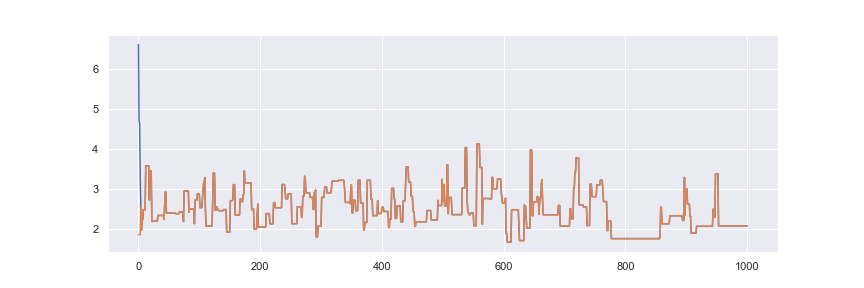
\includegraphics[width=6cm,height=2.5cm]{doublecoupling_pack/doublecoupling_sigma_chain_meeting}
			\vspace{0.2cm}
			{	\scriptsize \textbf{Samplings from all accepted chains }}\\
			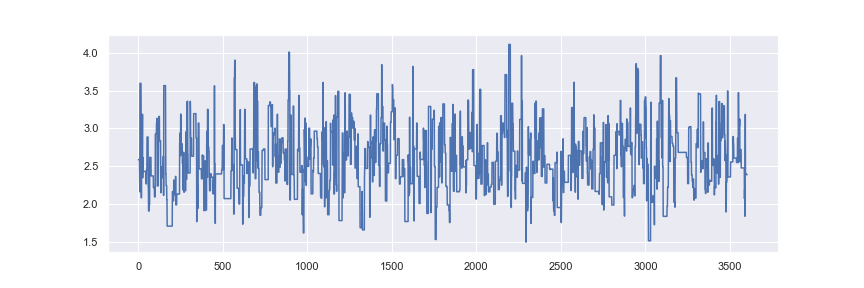
\includegraphics[width=6cm,height=2.5cm]{doublecoupling_pack/doublecoupling_sampling_sigma}
			%						%	
		\end{column}
		\begin{column}{0.4\textwidth}
			{\scriptsize \textbf{Sampling histogram with estimated distribution}}\\
			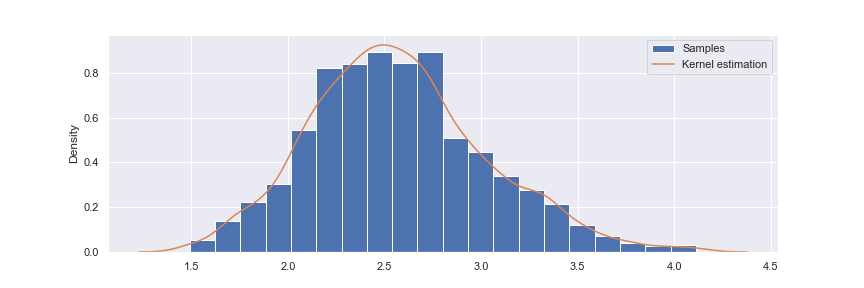
\includegraphics[width=5cm,height=5cm]{doublecoupling_pack/doublecoupling_sigma_histogram_kernel}
		\end{column}
	\end{columns}
	
\end{frame}
	\begin{frame}{Bibliography}
	\nocite{*}
	\bibliographystyle{unsrt}
	\tiny{ \bibliography{refs_MCMC,refs_ABC} }
\end{frame}
\end{document}
